\documentclass[tikz,border=10pt]{standalone}
\usepackage{tkz-euclide} % 增强几何绘图宏包

\begin{document}
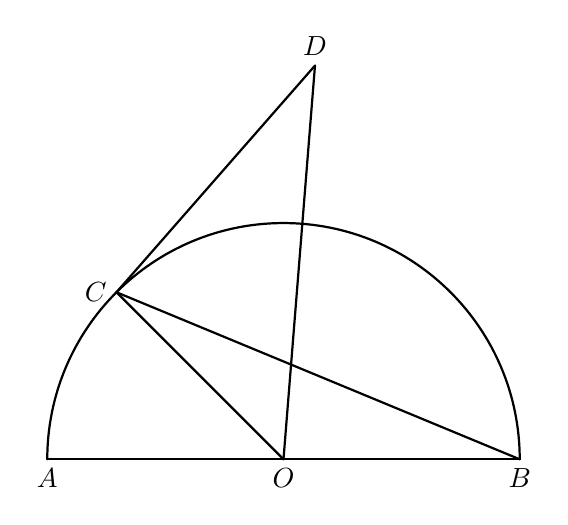
\begin{tikzpicture}[scale=2, line cap=round, line join=round]
    % 1. 定义基本参数
    \pgfmathsetmacro{\r}{1.5} % 圆半径
    
    % 2. 定义核心点坐标
    \coordinate (O) at (0,0);
    \coordinate (A) at (-\r,0);
    \coordinate (B) at (\r,0);
    
    % 定义 C 点（在圆弧上，取 135 度方向）
    \coordinate (C) at (135:\r);
    
    % 定义 D 点（基于几何推导，通常 OD 垂直于 AB）
    % 这里根据原图比例设置 D 点坐标
    \coordinate (D) at (0.2, 2.5); 

    % 3. 绘制图形元件
    % 绘制半圆弧 (从 0 到 180 度)
    \draw[thick] (B) arc (0:180:\r);
    
    % 绘制直径线段 AB
    \draw[thick] (A) -- (B);
    
    % 绘制内部连接线
    \draw[thick] (O) -- (C); % 半径 OC
    \draw[thick] (B) -- (C); % 弦 BC
    \draw[thick] (C) -- (D); % 线段 CD
    \draw[thick] (O) -- (D); % 线段 OD

    % 4. 标注点名称
    % 使用 pos 或 anchor 确保文字不遮挡线条
    \node[below] at (O) {$O$};
    \node[below] at (A) {$A$};
    \node[below] at (B) {$B$};
    \node[left] at (C) {$C$};
    \node[above] at (D) {$D$};

    % 5. (可选) 绘制直角标记，如果 D 在 O 的正上方
    % \draw (0.1,0) -- (0.1,0.1) -- (0,0.1); 

\end{tikzpicture}
\end{document}